\input cwebmac

% jafco
\input miniltx
\input graphicx


\nocon % omit table of contents
\datethis % print date on listing


\N{1}{1}Introduction. This is the firmware portion of Jaw and Fire control.

This will facilitate two actions: opening the jaw to release the floating
object and light the target on fire.

The jaw will close by return-spring so the action will to open it.

Fire is a  sequence of opening the jaw, releasing the butane and firing the
ignitor.

\vskip 4 pc
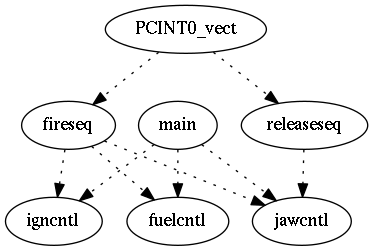
\includegraphics[width=35 pc]{jafco.png}

Extensive use was made of the datasheet, Atmel ``Atmel ATtiny25, ATtiny45,
ATtiny85 Datasheet'' Rev. 2586Q–AVR–08/2013 (Tue 06 Aug 2013 03:19:12 PM
EDT)
and ``AVR130: Setup and Use the AVR Timers'' Rev. 2505A–AVR–02/02.
\Y\B\X4:Include\X\6
\X5:Prototypes\X\6
\X6:Global variables\X\par
\fi

\M{2}\PB{\.{"F\_CPU"}} is used to convey the Trinket clock rate.
\Y\B\4\D$\.{F\_CPU}$ \5
\T{8000000\$U\$L}\par
\fi

\M{3}Here are some Boolean definitions that are used.
\Y\B\4\D$\.{ON}$ \5
\T{1}\par
\B\4\D$\.{OFF}$ \5
\T{0}\par
\B\4\D$\.{OPEN}$ \5
\T{1}\par
\B\4\D$\.{CLOSE}$ \5
\T{0}\par
\B\4\D$\.{SET}$ \5
\T{1}\par
\B\4\D$\.{CLEAR}$ \5
\T{0}\par
\fi

\M{4}\B\X4:Include\X${}\E{}$\6
\8\#\&{include} \.{<avr/io.h>}\SHC{ need some port access }\6
\8\#\&{include} \.{<util/delay.h>}\SHC{ need to delay }\6
\8\#\&{include} \.{<avr/interrupt.h>}\SHC{ have need of an interrupt }\6
\8\#\&{include} \.{<avr/sleep.h>}\SHC{ have need of sleep }\6
\8\#\&{include} \.{<avr/wdt.h>}\SHC{ have need of watchdog }\6
\8\#\&{include} \.{<stdlib.h>}\6
\8\#\&{include} \.{<stdint.h>}\par
\U1.\fi

\M{5}\B\X5:Prototypes\X${}\E{}$\6
\&{void} \\{jawcntl}(\\{uint8\_t}\\{state});\SHC{ Jaw open and close }\6
\&{void} \\{fuelcntl}(\\{uint8\_t}\\{state});\SHC{ Fuel on and off }\6
\&{void} \\{igncntl}(\\{uint8\_t}\\{state});\SHC{ on and off }\6
\&{void} \\{releaseseq}(\&{void});\6
\&{void} \\{fireseq}(\&{void});\par
\U1.\fi

\M{6}
My lone global variable is a function pointer.
This lets me pass arguments to the actual interrupt handlers, should I need to.
This pointer gets the appropriate function attached by one of the \PB{%
\.{"ISR()"}}
functions.

\Y\B\4\X6:Global variables\X${}\E{}$\6
\&{void} ${}({*}\\{handleirq})(\,)\K\NULL{}$;\6
\&{int} \\{main}(\&{void})\1\1\6
$\{{}$\6
\X26:Initialize interrupts\X\6
\X25:Initialize pin inputs\X\6
\X24:Initialize pin outputs\X\par
\U1.\fi

\M{7}
Of course, any interrupt function requires that bit ``Global Interrupt Enable''
is set; usually done through calling sei(). Doing this after the pin setup is
the best time.
\Y\B\\{sei}(\,);\par
\fi

\M{8}
Rather than burning loops, waiting for something to happen,
the ``sleep'' mode is used.
The specific type of sleep is `idle'.
In idle, execution stops but timers continue.
Interrupts are used to wake it.
\Y\B\X32:Configure to wake upon interrupt\X\par
\fi

\M{9}
This is the loop that does the work.
It should spend most of its time in \PB{\\{sleep\_mode}},
comming out at each interrupt event.

\Y\B\&{for} ( ;  ; \,)\6
$\{{}$\par
\fi

\M{10}
We don't want anything cooking while we are asleap.
\Y\B\\{igncntl}(\.{OFF});\6
\\{fuelcntl}(\.{OFF});\6
\\{jawcntl}(\.{CLOSE});\par
\fi

\M{11}
Now we wait in ``idle'' for any interrupt event.
\Y\B\\{sleep\_mode}(\,);\par
\fi

\M{12}
If execution arrives here, some interrupt has been detected.
\Y\B\&{if} ${}(\\{handleirq}\I\NULL{}$)\SHC{ not sure why it would be, but to
be safe }\6
${}\{{}$\1\6
\\{handleirq}(\,);\6
${}\\{handleirq}\K\NULL{}$;\SHC{ reset so that the action cannot be repeated }\6
\4${}\}{}$\SHC{ end if handleirq }\2\6
$\}{}$\SHC{ end for }\6
\&{return} \T{0};\SHC{ it's the right thing to do! }\6
$\}{}$\SHC{ end main() }\par
\fi

\N{1}{13}Interrupt Handling.

\Y\B\&{void} \\{releaseseq}(\,)\1\1\6
$\{{}$\par
\fi

\M{14}
This sequence will proceed only while the button is held.
\Y\B\\{jawcntl}(\.{OPEN});\6
\&{while} ${}(\R(\.{PINB}\AND(\T{1}\LL\.{PB3}))){}$\1\5
\\{\_delay\_ms}(\T{10});\2\6
\\{jawcntl}(\.{CLOSE}); $\}{}$\par
\fi

\M{15}


\Y\B\&{void} \\{fireseq}(\,)\1\1\6
$\{{}$\6
\\{uint8\_t}\\{firingstate};\7
\&{enum} \&{firingstates} ${}\{{}$\1\6
${}\\{ready},\39\\{opened},\39\\{igniting},\39\\{burning},\39\\{cooling}{}$\2\6
${}\};{}$\7
${}\\{firingstate}\K\\{ready}{}$;\par
\fi

\M{16}
This sequence will proceed only while the button is held.
It can terminate after any state.
\PB{\.{"\_delay\_ms()"}} is a handy macro good for $2^{16}$ milliseconds of
delay.
\Y\B\&{while} ${}(\R(\.{PINB}\AND(\T{1}\LL\.{PB4})))$ $\{{}$\par
\fi

\M{17}
The jaw opens here for fire.
\Y\B\&{if} ${}(\\{firingstate}\E\\{ready}){}$\5
${}\{{}$\1\6
\\{jawcntl}(\.{OPEN});\6
${}\\{firingstate}\K\\{opened};{}$\6
\&{continue};\6
\4${}\}{}$\2\par
\fi

\M{18}
Ignitor is on.
\Y\B\&{if} ${}(\\{firingstate}\E\\{opened}){}$\5
${}\{{}$\1\6
\\{igncntl}(\.{ON});\6
${}\\{firingstate}\K\\{igniting};{}$\6
\&{continue};\6
\4${}\}{}$\2\par
\fi

\M{19}
Fuel opens.
\Y\B\&{if} ${}(\\{firingstate}\E\\{igniting}){}$\5
${}\{{}$\1\6
\\{fuelcntl}(\.{ON});\6
${}\\{firingstate}\K\\{burning};{}$\6
\&{continue};\6
\4${}\}{}$\2\6
\\{\_delay\_ms}(\T{10}); $\}{}$\par
\fi

\M{20}
Once the loop fails we set fuel and ignitor off and close the jaw.
\Y\B\\{igncntl}(\.{OFF});\6
\\{fuelcntl}(\.{OFF});\6
\\{\_delay\_ms}(\T{5000});\6
\\{jawcntl}(\.{CLOSE}); $\}{}$\par
\fi

\N{1}{21}The ISRs.

The ISRs are pretty skimpy as they mostly used to point \PB{\\{handleirq}(\,)}
to
the correct function.
The need for global variables is minimized.

\fi

\M{22}
This vector responds to the jaw input at pin PB3 or fire input at PB4.
A simple debounce is included.
\Y\B\.{ISR}(\\{PCINT0\_vect})\6
${}\{{}$\1\6
\&{const} \\{int8\_t}\\{high}${}\K\T{32};{}$\6
\&{const} \\{int8\_t}\\{low}${}\K{-}\\{high};{}$\7
${}\\{int8\_t}\\{dbp3}\K\T{0};{}$\6
${}\\{int8\_t}\\{dbp4}\K\T{0};{}$\6
\&{while} ${}(\\{abs}(\\{dbp3})<\\{high}){}$\5
${}\{{}$\1\6
\&{if} ${}(\R(\.{PINB}\AND(\T{1}\LL\.{PB3}))\W\\{dbp3}>\\{low}){}$\1\5
${}\\{dbp3}\MM;{}$\2\6
\&{else} \&{if} ${}((\.{PINB}\AND(\T{1}\LL\.{PB3}))\W\\{dbp3}<\\{high}){}$\1\5
${}\\{dbp3}\PP;{}$\2\6
\\{\_delay\_ms}(\T{1});\6
\4${}\}{}$\2\6
\&{while} ${}(\\{abs}(\\{dbp4})<\\{high}){}$\5
${}\{{}$\1\6
\&{if} ${}(\R(\.{PINB}\AND(\T{1}\LL\.{PB4}))\W\\{dbp4}>\\{low}){}$\1\5
${}\\{dbp4}\MM;{}$\2\6
\&{else} \&{if} ${}((\.{PINB}\AND(\T{1}\LL\.{PB4}))\W\\{dbp4}<\\{high}){}$\1\5
${}\\{dbp4}\PP;{}$\2\6
\\{\_delay\_ms}(\T{1});\6
\4${}\}{}$\2\6
\&{if} ${}(\\{dbp3}\E\\{low}){}$\1\5
${}\\{handleirq}\K{\AND}\\{releaseseq};{}$\2\6
\&{else} \&{if} ${}(\\{dbp4}\E\\{low}){}$\1\5
${}\\{handleirq}\K{\AND}\\{fireseq};{}$\2\6
\4${}\}{}$\2\par
\fi

\N{1}{23}These are the supporting routines, procedures and configuration
blocks.


Here is the block that sets-up the digital I/O pins.
\fi

\M{24}\B\X24:Initialize pin outputs\X${}\E{}$\6
${}\{{}$\C{ set the jaw port direction }\1\6
${}\.{DDRB}\MRL{{\OR}{\K}}(\T{1}\LL\.{DDB0}){}$;\C{ set the fuel port direction
}\6
${}\.{DDRB}\MRL{{\OR}{\K}}(\T{1}\LL\.{DDB1}){}$;\C{ set the ignition port
direction }\6
${}\.{DDRB}\MRL{{\OR}{\K}}(\T{1}\LL\.{DDB2});{}$\6
\4${}\}{}$\2\par
\U6.\fi

\M{25}\B\X25:Initialize pin inputs\X${}\E{}$\6
${}\{{}$\C{ set the jaw input pull-up }\1\6
${}\.{PORTB}\MRL{{\OR}{\K}}(\T{1}\LL\.{PORTB3}){}$;\C{ set the fire input
pull-up }\6
${}\.{PORTB}\MRL{{\OR}{\K}}(\T{1}\LL\.{PORTB4});{}$\6
\4${}\}{}$\2\par
\U6.\fi

\M{26}\B\X26:Initialize interrupts\X${}\E{}$\6
${}\{{}$\C{ enable  change interrupt for jaw input }\1\6
${}\.{PCMSK}\MRL{{\OR}{\K}}(\T{1}\LL\.{PCINT3}){}$;\C{ enable  change interrupt
for fire input }\6
${}\.{PCMSK}\MRL{{\OR}{\K}}(\T{1}\LL\.{PCINT4}){}$;\C{ General interrupt Mask
register }\6
${}\.{GIMSK}\MRL{{\OR}{\K}}(\T{1}\LL\.{PCIE});{}$\6
\4${}\}{}$\2\par
\U6.\fi

\M{27}
Here is a simple procedure to operate the jaw.
\Y\B\&{void} \\{jawcntl}(\\{uint8\_t}\\{state})\6
${}\{{}$\1\6
${}\.{PORTB}\K\\{state}\?\.{PORTB}\OR(\T{1}\LL\.{PORTB0}):\.{PORTB}\AND\CM(%
\T{1}\LL\.{PORTB0});{}$\6
\4${}\}{}$\2\par
\fi

\M{28}
Here is a simple procedure to operate the fuel.
\Y\B\&{void} \\{fuelcntl}(\\{uint8\_t}\\{state})\6
${}\{{}$\1\6
${}\.{PORTB}\K\\{state}\?\.{PORTB}\OR(\T{1}\LL\.{PORTB1}):\.{PORTB}\AND\CM(%
\T{1}\LL\.{PORTB1});{}$\6
\4${}\}{}$\2\par
\fi

\M{29}
Here is a simple procedure to operate the ignition.
\Y\B\&{void} \\{igncntl}(\\{uint8\_t}\\{state})\6
${}\{{}$\1\6
${}\.{PORTB}\K\\{state}\?\.{PORTB}\OR(\T{1}\LL\.{PORTB2}):\.{PORTB}\AND\CM(%
\T{1}\LL\.{PORTB2});{}$\6
\4${}\}{}$\2\par
\fi

\M{30}
See section the datasheet for details on the Watchdog Timer.
We are not using it right now.
\fi

\M{31}\B\X31:Initialize watchdog timer\X${}\E{}$\6
${}\{{}$\1\6
${}\.{WDTCR}\MRL{{\OR}{\K}}(\T{1}\LL\.{WDCE})\OR(\T{1}\LL\.{WDE});{}$\6
${}\.{WDTCR}\K(\T{1}\LL\.{WDIE})\OR(\T{1}\LL\.{WDP2}){}$;\SHC{ reset after
about 0.25 seconds }\6
\4${}\}{}$\2\par
\fi

\M{32}
Setting these bits configure sleep\_mode() to go to ``idle''.
Idle allows the counters and comparator to continue during sleep.

\Y\B\4\X32:Configure to wake upon interrupt\X${}\E{}$\6
${}\{{}$\1\6
${}\.{MCUCR}\MRL{\AND{\K}}\CM(\T{1}\LL\.{SM1});{}$\6
${}\.{MCUCR}\MRL{\AND{\K}}\CM(\T{1}\LL\.{SM0});{}$\6
\4${}\}{}$\2\par

\U8.\fi


\inx
\fin
\con
